\documentclass[10pt, compress]{beamer}

\usetheme{m}

\usepackage{booktabs}
\usepackage{amsmath,amsfonts,amsthm,commath,bm}
\DeclareMathOperator*{\plim}{plim}
\DeclareMathOperator{\Var}{Var}
\DeclareMathOperator{\E}{\mathbb{E}}
\newcommand{\that}{\hat{\theta}}

\title{Potentials and Perils of Preprocessing}
\subtitle{Alexander W. Blocker and Xiao-Li Meng}
\date{April 9th, 2015}
\author{Maxime and Angela}


\begin{document}
\maketitle

\begin{frame}[fragile]
    \frametitle{Overview of the Paper}
    
    Addresses data preprocessing and its effect on later analysis in two main ways:
    \begin{enumerate}
    \item Points out potential problems with current preprocessing strategies
    \item Describes a statistical framework for analyzing data preprocessing
    \end{enumerate}

\end{frame}

\begin{frame}[fragile]
    \frametitle{What is the Preprocessing problem?}

    Raw data is reduced based on assumptions about future analysis, which \textbf{constrains downstream data analysis}.
    
    Yet, preprocessing is necessary:

    \begin{enumerate}
    \item Even if original data was passed down, many users may not know how to process the data themselves. 
    \item The analyst performing the preprocessing may have detailed knowledge about the experimental situation that the data user does not have
  \end{enumerate}
  
\end{frame}

\begin{frame}[fragile]
    \frametitle{The Multiphase Setup}

    Two phases:
    \begin{enumerate}
    \item \textbf{Preprocessing} = Data generation, collection, preprocessing
    \item \textbf{Downstream Analysis} = inference using output from phase 1
    \end{enumerate}
    
    \begin{figure}[h!]
    \centering
    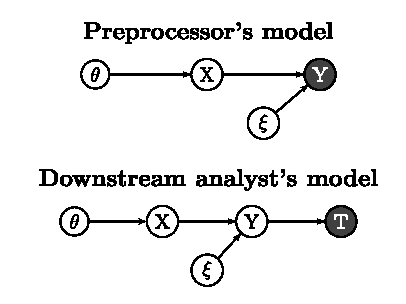
\includegraphics[width=.6\textwidth]{assets/two_phase_setting.ps}
    \end{figure}

\end{frame}

\begin{frame}[fragile]
    \frametitle{Missing Data}
    \begin{figure}[h!]
    \centering
    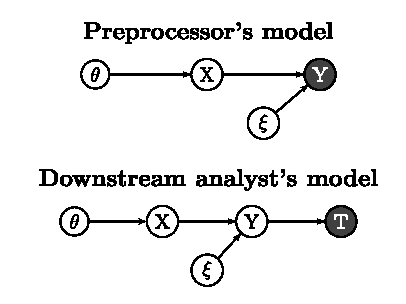
\includegraphics[width=.5\textwidth]{assets/two_phase_setting.ps}
    \end{figure}   
    \begin{enumerate}
    \item \textbf{Missingness from data generation: X is missing} since preprocessor observes Y
    \item \textbf{Missingness from inference process: Y and X are both missing} since data analyst observes T
    \end{enumerate}
    
    Note that the analyst's $T(Y)$ is a product of preprocessing, so it is a \textbf{design decision} of the preprocessor.

\end{frame}

\begin{frame}[fragile]
    \frametitle{Square Kilometer Array}
    \begin{columns}
        \column{0.5\textwidth}
            \begin{itemize}
                \item Radio telescope to be built around 2018-2030
                \item Total collecting area = $1~\mathrm{km}^2$, between about 3000 dishes.
                \item Raw data: Each antenna produces \textbf{420Gb/s}
            \end{itemize}
        \column{0.5\textwidth}
            \vspace{.01cm}
            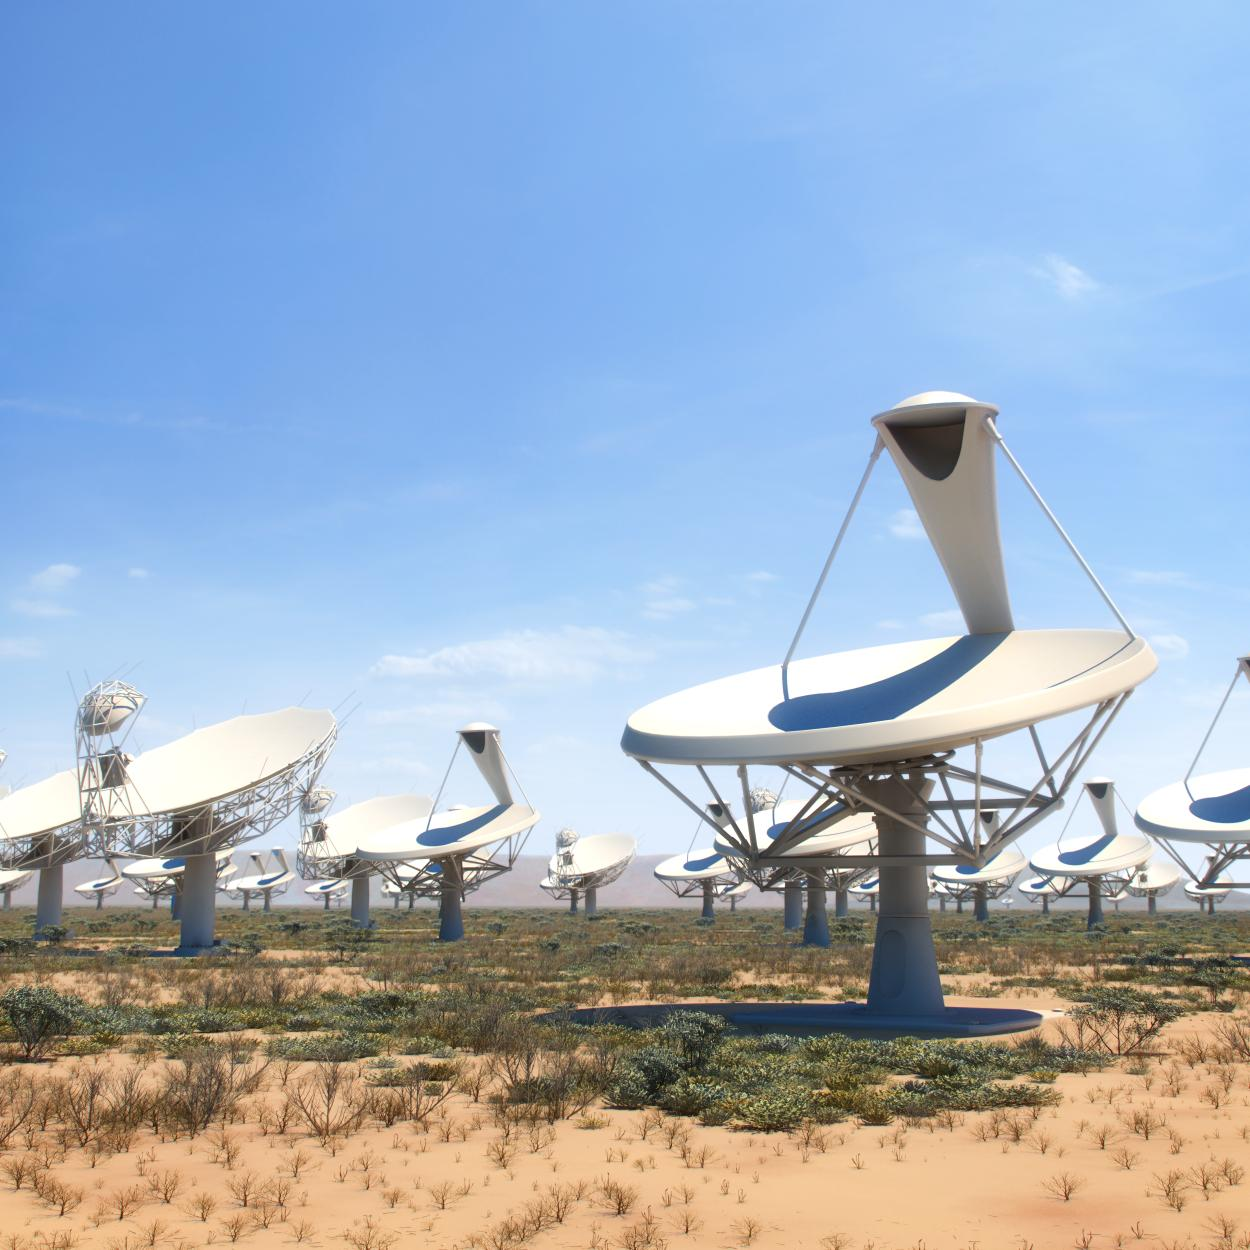
\includegraphics[height=\textheight]{assets/ska_dish_mid_africa_closeup.jpg}
    \end{columns}
\end{frame}
\begin{frame}[fragile]
    \frametitle{Square Kilometer Array}
    \begin{columns}
        \column{0.5\textwidth}
            \begin{itemize}
                \item First stage preprocessing: correlation of signals between dishes
                \item \textbf{Lossless} reduction to about 100~Tb/s ($\approx$~the internet)
                \item Standard lossless compression algorithms (SZIP, GZIP…) can further reduce the data by about a third (Rajeswaran \& Winberg 2013).
            \end{itemize}
        \column{0.5\textwidth}
            \vspace{.01cm}
            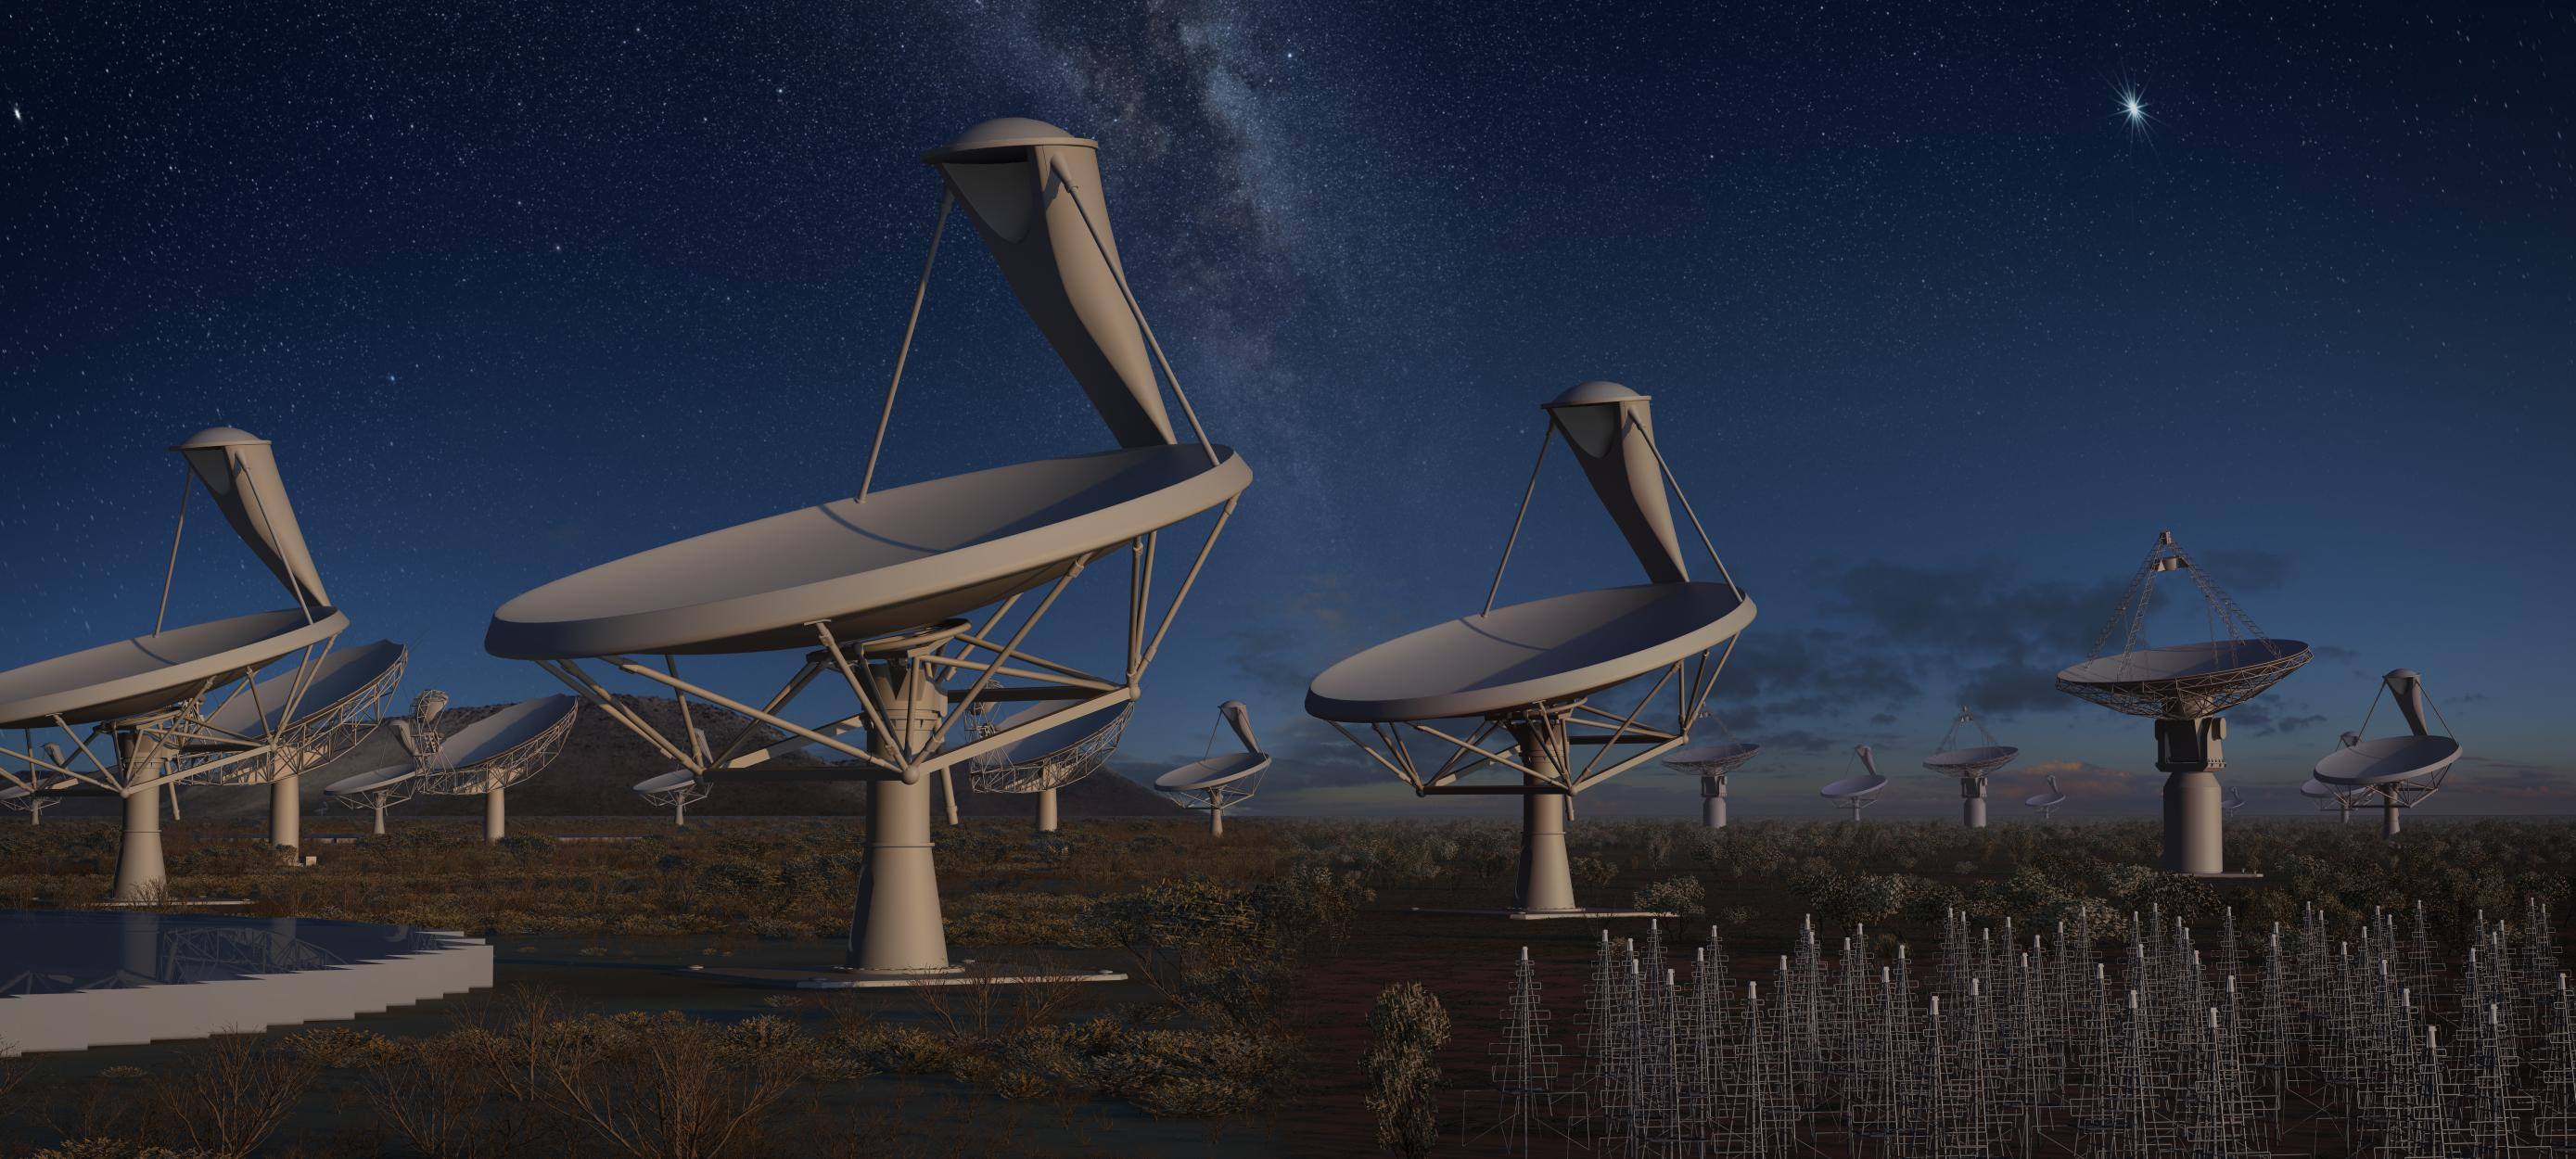
\includegraphics[height=\textheight]{assets/skaall_night.jpg}
    \end{columns}
\end{frame}
\begin{frame}[fragile]
    \frametitle{Square Kilometer Array}
    \begin{columns}
        \column{0.5\textwidth}
            \begin{itemize}
                \item That's still more raw data than is reasonable to store on hard drives
                \item it will be necessary to \textbf{further reduce} the data in \textbf{real time}
            \end{itemize}
        \column{0.5\textwidth}
            \vspace{.01cm}
            \centering
            \includegraphics[height=\textheight]{assets/sky_survey.ps}
    \end{columns}
\end{frame}
\begin{frame}[fragile]
    \frametitle{Square Kilometer Array}
    \begin{figure}[h!]
    \centering
    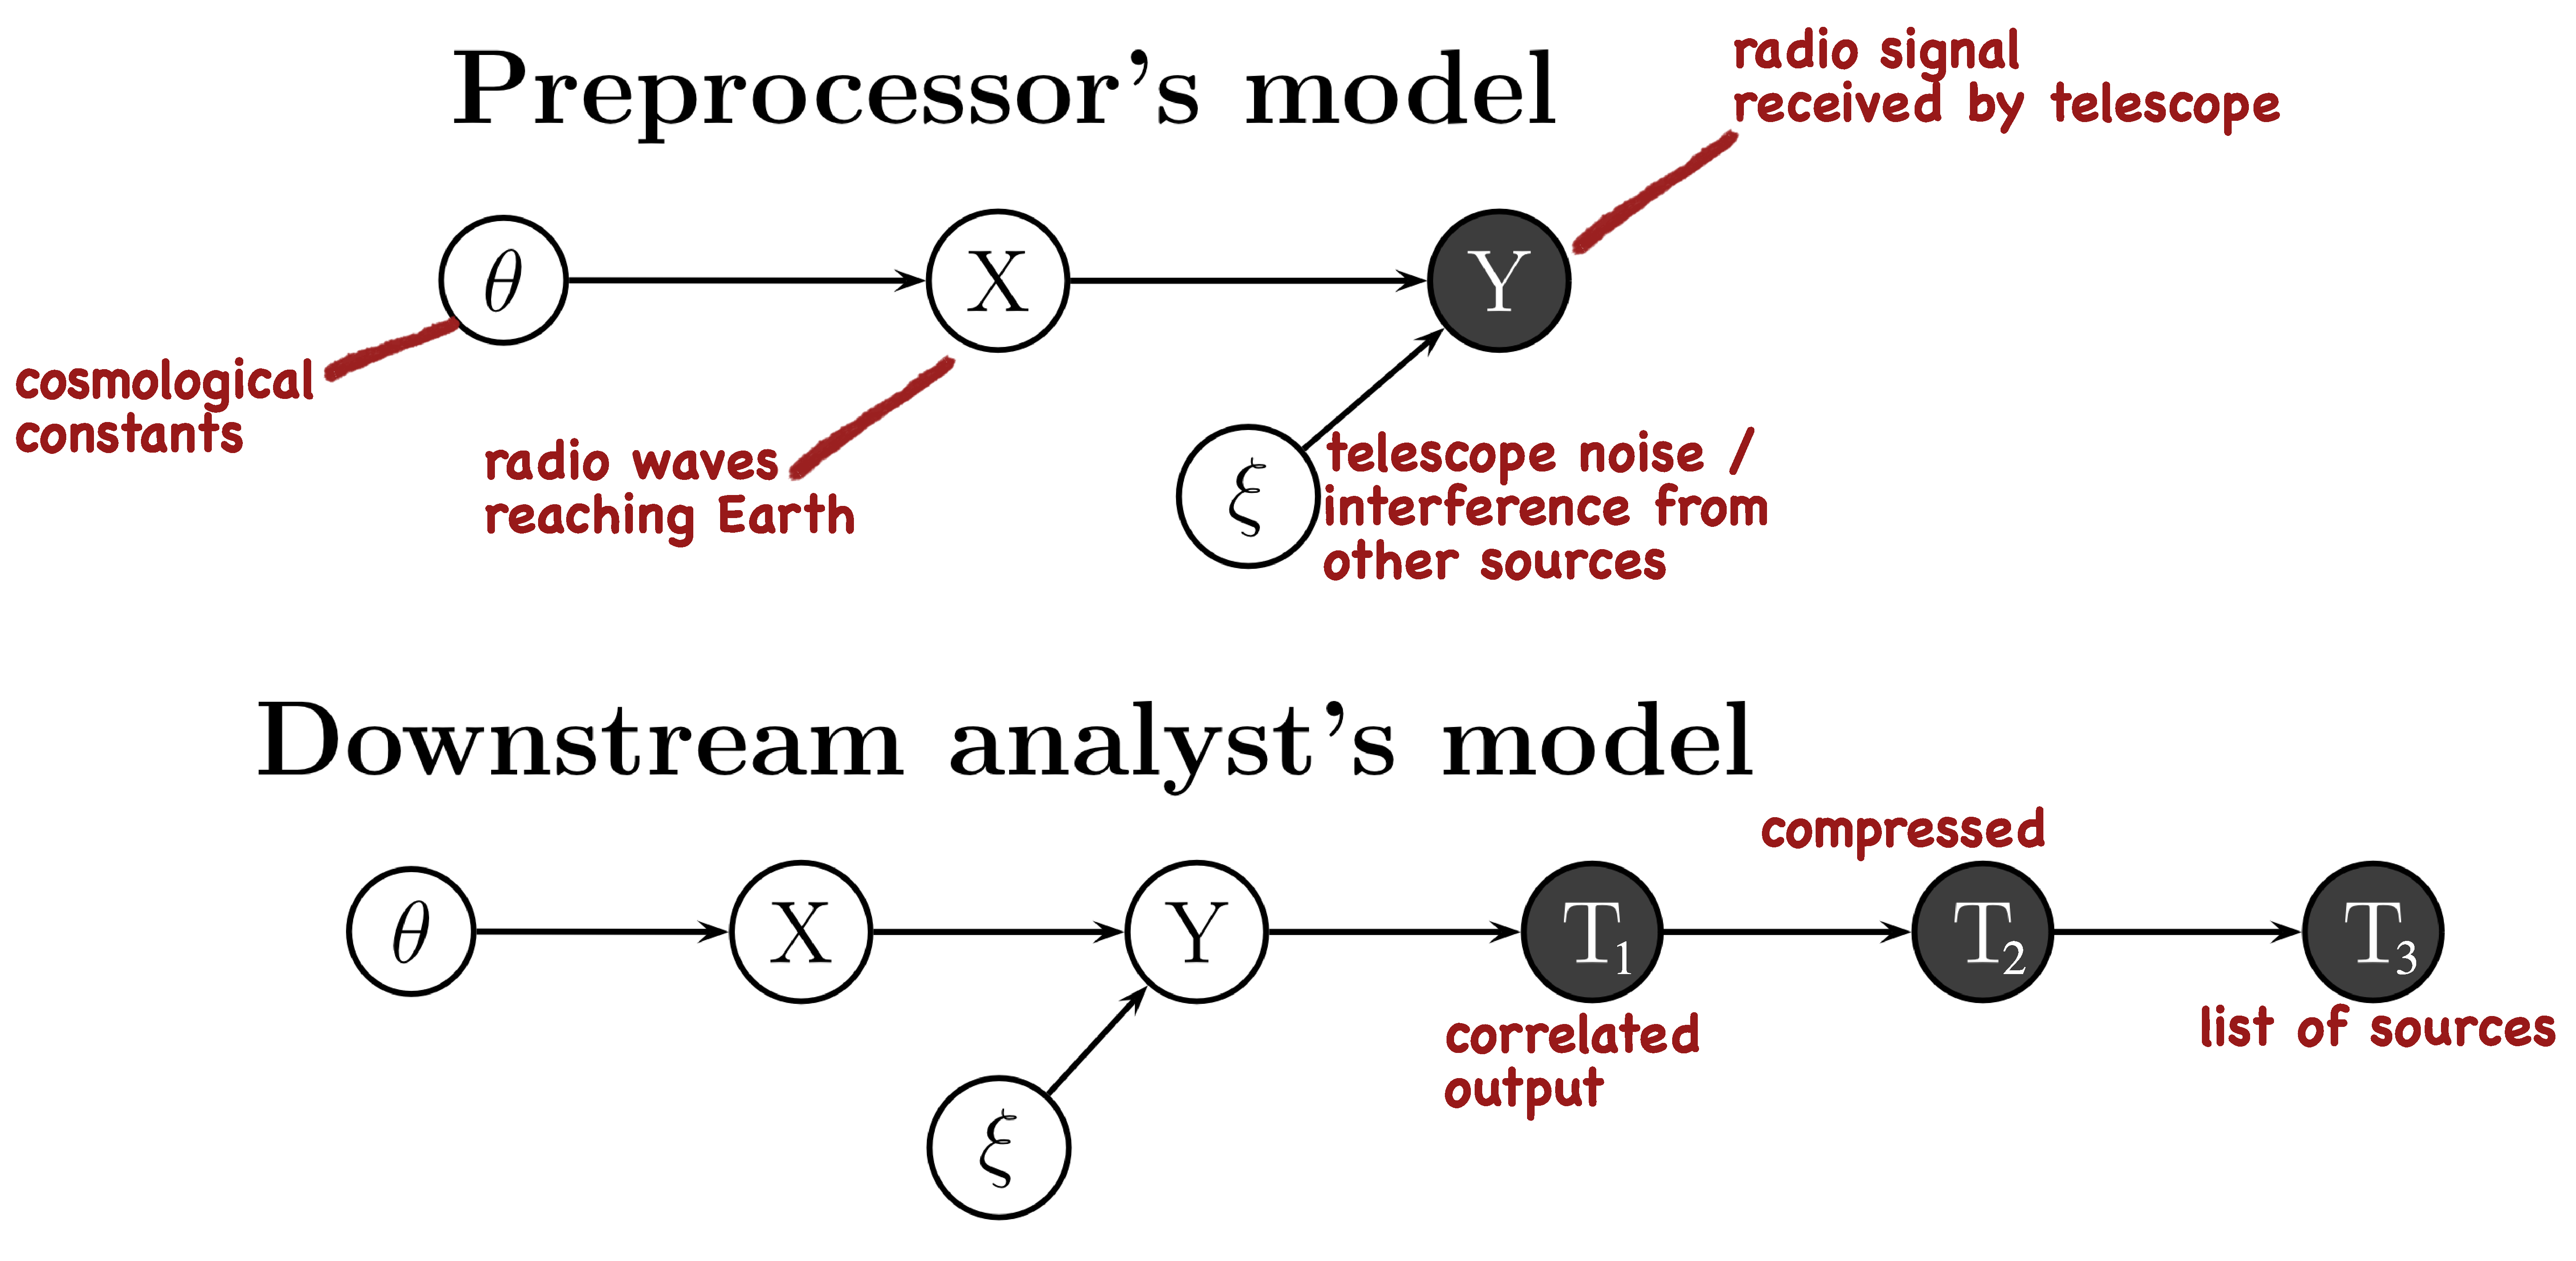
\includegraphics[width=\textwidth]{assets/radio_observation_model.eps}
    \end{figure}   
    \begin{itemize}
        \item 3 possible levels of preprocessing
    \end{itemize}
\end{frame}
\begin{frame}[fragile]
    \frametitle{High-throughput Biology: Expression Microarrays}
    
    \begin{columns}
        \column{0.5\textwidth}
            \begin{itemize}
                \item \textbf{Raw data} are probe intensity measurements
                \item \textbf{Want to study} log fold change in gene expression between different conditions
            \end{itemize}
        \column{0.5\textwidth}
        \vspace{.01cm}
            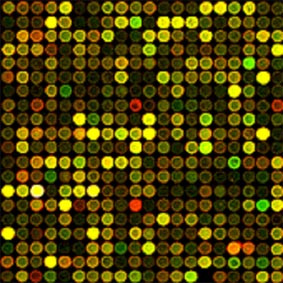
\includegraphics[height=\textheight]{assets/microarray.jpg}
    \end{columns}
    
\end{frame}

\begin{frame}[fragile]
    \frametitle{High-throughput Biology: Expression Microarrays}
    
    \textbf{Many levels of preprocessing:} 

    \begin{enumerate}
    \item \textbf{background correction} to reduce noise- many different algorithms, mostly passing down point estimates
    \vspace*{5mm}
    \item \textbf{normalization across different microarrays} to reduce systematic error
    \vspace*{5mm}
    \item screening for data corruption, etc.
    \end{enumerate}
    
\end{frame}

\begin{frame}[fragile]
    \frametitle{High-throughput Biology: Expression Microarrays}
    Let's say our goal is to assess if there is a significant difference in expression levels of 10 different genes between people
    who have blue eyes and people who have brown eyes

    \centering
    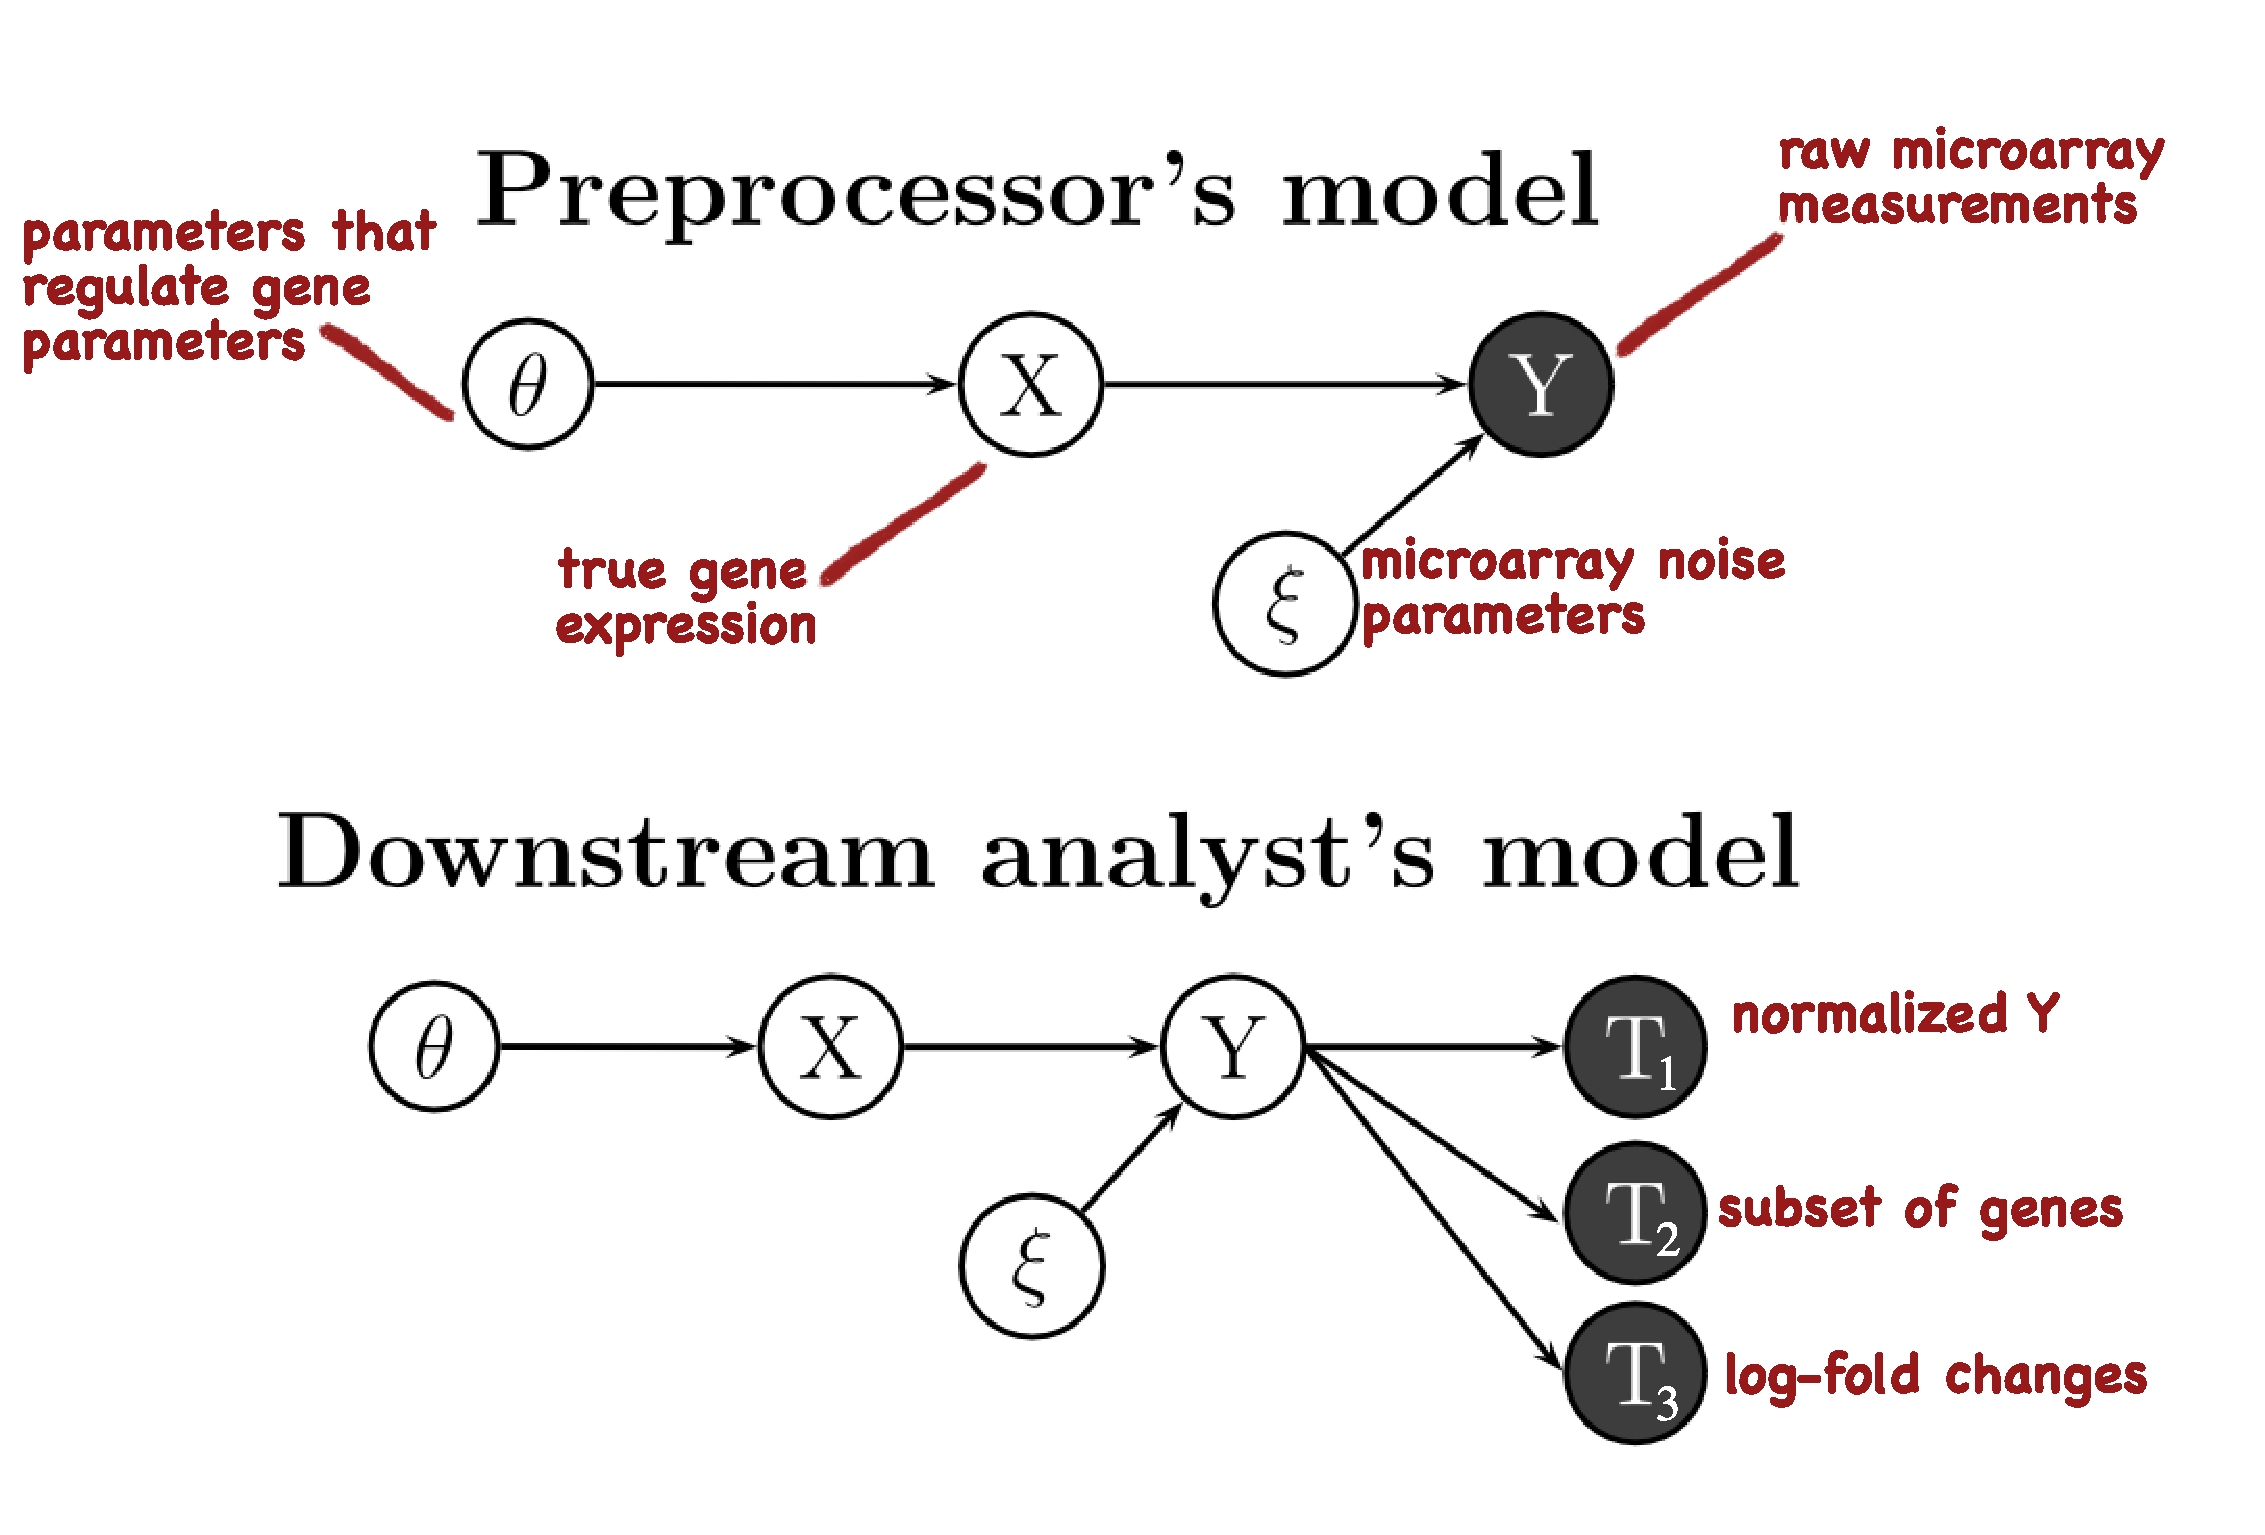
\includegraphics[width=0.9\textwidth]{assets/dna_model.eps}

    %$\theta$ = gene regulatory parameters that govern gene expression
    %$X$ = true gene expression levels of these 10 genes, and phenotypic observation if the person has blue eyes or brown eyes
    %$\xi$ = microarray noise parameters (such as hybridization, variance of experimental conditions, bleeding, clarity of signal, etc.)
    %$Y$ = raw probe measurements from the microarray
    %$T$ = normalized, transformed, reduced-dimension gene expression measurements for each of the 10 genes

\end{frame}


\begin{frame}[fragile]
    \frametitle{Why are Preprocessing and Analysis separate?}
    
    \begin{enumerate} 
    \item \textbf{Data warehousing limitations}- cannot store the amount of data produced by radio telescopes
    \vspace*{3mm}
    \item \textbf{Division of labor}- 
        \begin{itemize}
        \item inefficient for each biologist to reproduce a whole analysis pipeline 
        \item many companies that provide microarrays include algorithms and methods for data preprocessing immediately from raw output
        \end{itemize}
    \vspace*{3mm}
    \item \textbf{Inability to provide whole datasets, only preprocessed versions}- data anonimization concerns, for example
    \end{enumerate}

\end{frame}

\begin{frame}[fragile]
    \frametitle{What should we retain?}
    \begin{itemize}
        \item \textbf{Optimal:} lossless compression to \textbf{minimal sufficient} statistic for a given research model
            \begin{itemize}
                \item Sufficiency: $\Pr\del{\theta \mid Y,T\del{Y}}=\Pr\del{\theta \mid T\del{Y}}$
                \item This is only practical if the analyst's model $X \mid \theta$ is specified and known before preprocessing.
            \end{itemize}
        \item \textbf{More realistic:} Hope downstream analyst's scientific model is related (congenial) to preprocessor's observation model
    \end{itemize}
\end{frame}

\begin{frame}[fragile]
    \frametitle{What should we retain?}
    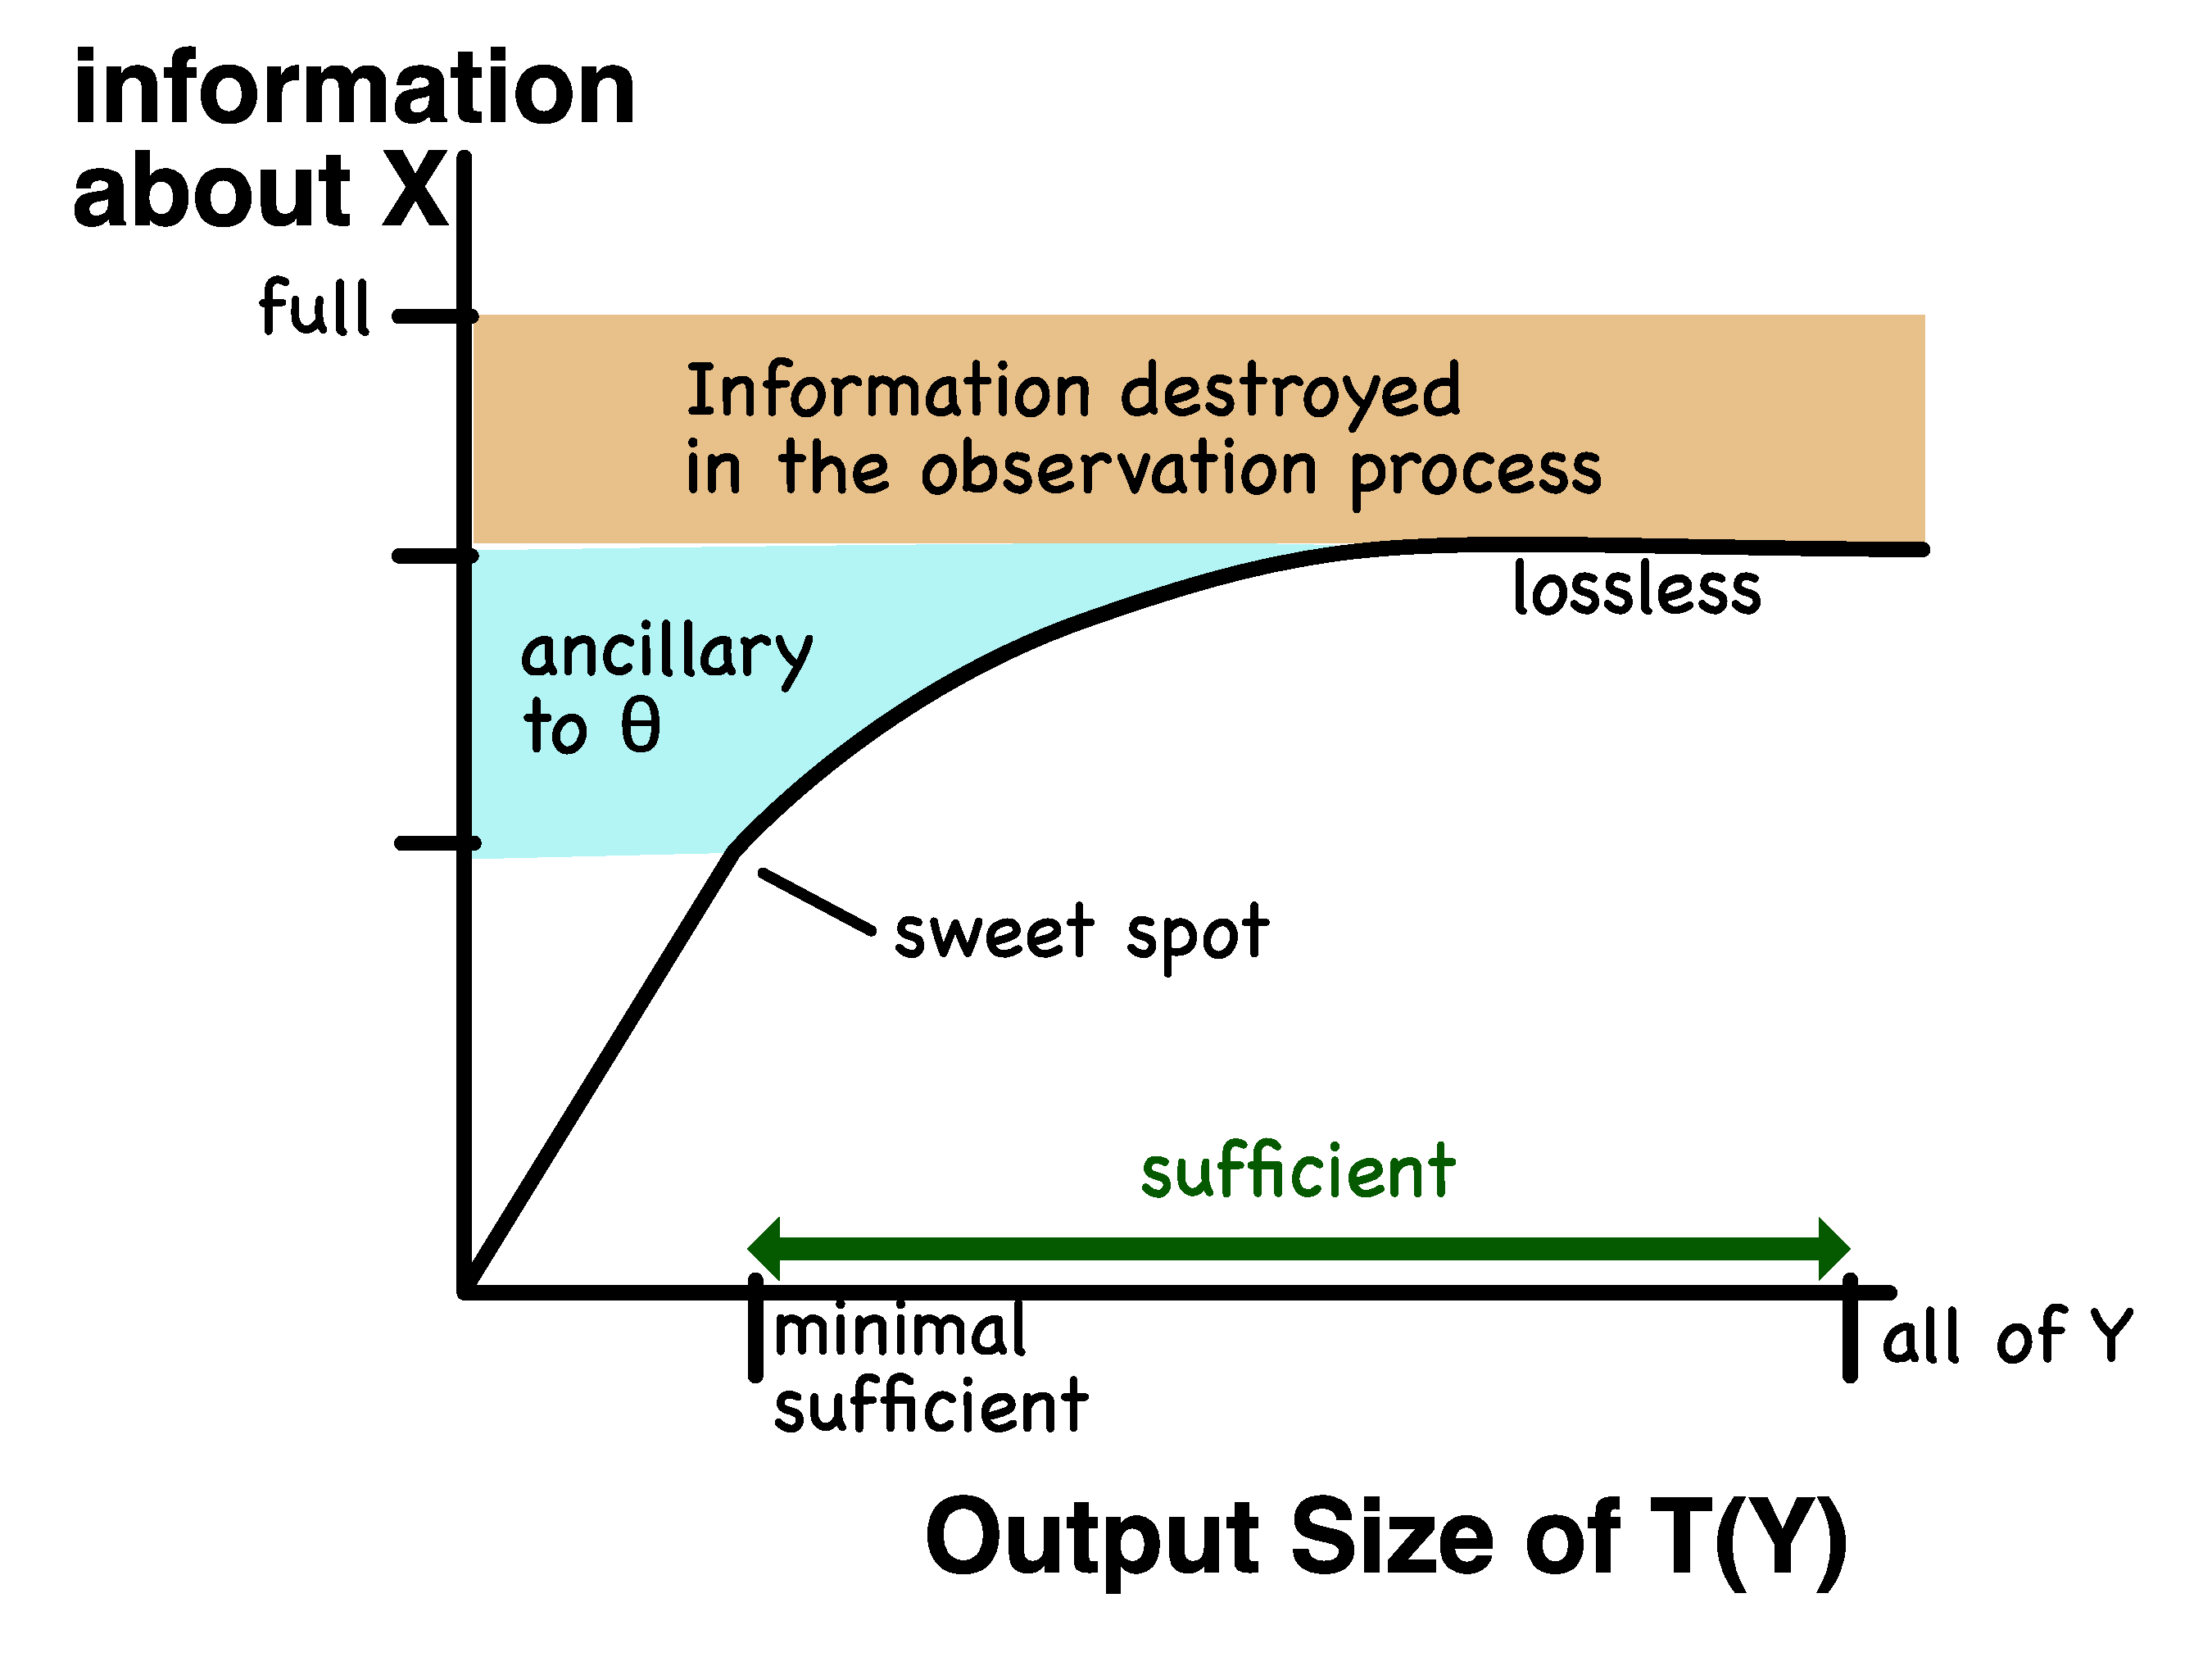
\includegraphics[width=\textwidth]{assets/information.eps}
\end{frame}


\begin{frame}[fragile]

    \frametitle{Regression with Nuisance Parameters: An Example}
    
    \vspace*{5mm}
    
    \textbf{Data:} Each processor $i$ observes $y_{ij} \sim N(\beta_0 + \beta_{1i}x_j, \sigma^2)$ for $j = 1 \ldots m$
    
    \vspace*{2mm}

    \textbf{Downstream analyst wants to estimate $\beta_0$}, with $\beta_{1i}$ and $\sigma^2$ as nuisance parameters so that $\xi$ = $(\sigma^2, \beta_{11} \ldots \beta_{1n})$
    
    \vspace*{2mm}

    \textbf{Preprocessor reduces data to:} $T_i = \frac{1}{m}\sum\del{y_{ij} - \hat{\beta_{ij}}x_j}$ where $\hat{\beta_{1i}}$ is the OLS estimator of $\beta_{1i}$.
    
    \vspace*{5mm}
    
    Distribution of $T_i$ still depends on $\sigma^2$, but is free of $B_{1i}$ 
\end{frame}

\begin{frame}[fragile]
    \frametitle{What should we retain?}
    \begin{itemize}
        \item \textbf{Problem:} The “sweet spot” depends on the scientific model $X \mid \theta$. Different analysts will have different models $X \mid \eta$ with a different optimal $\tilde{T}\del{Y}$
            \begin{itemize}
                \item and even those might not be known in advance.
            \end{itemize}
        \item \textbf{Goal:} Find a statistic that retains enough information to keep most people happy.
    \end{itemize}
\end{frame}

\begin{frame}[fragile]
    \frametitle{Decision theory to the rescue.}
    \begin{itemize}
        \item Further reduction is often necessary, but \textbf{comes at a cost}
        \item formalised through \textbf{decision theory}: loss function $L\del{ \hat{\theta}, \theta_{true}}$
        \item risk = expected loss 
            \[ 
                R\del{\hat{\theta},\theta_{true}} = \E{\cbr{L\del{ \hat{\theta}, \theta_{true}}}}
            \]
        \item regret = how bad is this estimator?
            \[
                R\del{\hat{\theta},\theta_{true}} - R\del{\hat{\theta}^*,\theta_{true}}
            \]
        \item Idea: risk with respect to better estimator. In our case, using the \textbf{full data} instead of the \textbf{reduced data}.
                \[
                    R\del{\that\del{T},\that\del{Y}} = \E{\cbr{L\del{ \that\del{T},\that\del{Y} }}}
                \]
    \end{itemize}
\end{frame}
\begin{frame}[fragile]
    \frametitle{Decision theory to the rescue.}
        \[
                R\del{\that\del{T},\that\del{Y}} = \E{\cbr{L\del{ \that\del{T},\that\del{Y} }}}
        \]
    \begin{itemize}
        \item e.g. mean-squared error
            \[
            R\del{\that\del{T},\that\del{Y}} = \E{\cbr{ \del{ \that\del{T}-\that\del{Y} }^2 }} 
            \]
        \item asymptotically $R\del{\that\del{T},\that\del{Y}} \rightarrow \mathrm{regret}$ (“asymptotic decorrelation”)
        \item for multiple analysts with different models, the costs can be averaged:
            \[
                \mathrm{regret}\del{T} = \frac{1}{N_{analysts}}\sbr{R\del{\that\del{T},\that\del{Y}}+R\del{\hat{\xi}\del{T},\hat{\xi}\del{Y}}+\ldots}
            \]
    \end{itemize}
\end{frame}


\begin{frame}[fragile]
    \frametitle{Projecting into the future}
    
    \textbf{Likelihood as a minimal sufficient statistic}- computationally efficient approximations of the likelihood function could be foundation for passing information between phases of downstream analysis.  
    
    Two things to consider:
    \begin{enumerate}
    \item Nuisance parameters 
    \item Downstream analysts may be constrained by the likelihood approximation chosen. For example, analysts may want to estimate the data and estimate the parameters, and going from likelihood approximation to estimates of the data, X, could require a lot of effort and computation.
    \end{enumerate}

\end{frame}

\begin{frame}[fragile]
    \frametitle{Connections to Multiple Imputation}
    
    \begin{enumerate}
    \item Relates to prior presentation on congeniality in MI
    \item Both papers want to bound and measure the amount of degradation in inference when information is imperfectly combined
    \item Congeniality paper concludes that nuisance parameters can be a stumbling block for MI, perhaps understanding role of preprocessing in addressing nuisance parameters could be helpful
    \end{enumerate}
    
\end{frame}

\begin{frame}[fragile]
    \frametitle{Conclusion}
    
    Despite previous discussion and historical concerns about data preprocessing, not much work has been done to address issues related with preprocessing.
    
    \vspace*{3mm}
    
    This paper has proposed a conceptual and mathematical framework to understand the issues that arise in preprocessing, and provides some suggestions for how researchers can begin to think about and investigate preprocessing effects. 
  
\end{frame}
\begin{frame}[fragile]
    \frametitle{References}
    
    \begin{enumerate}
        \item Babu, M. Madan. "An Introduction to Microarray Data Analysis." Microarray Data Analysis (2004).
    	\item Blocker, Alexander W., and Xiao-Li Meng. "The potential and perils of preprocessing: Building new foundations." Bernoulli 19.4 (2013): 1176-1211.
		\item Rajeswaran, Karthik, and Simon Winberg. "Lossless Compression of SKA Data Sets." Communications and Network 2013 (2013).
	\end{enumerate}
  
\end{frame}


\end{document}
